\section{Техническое задание}
\subsection{Основание для разработки}

Основанием для разработки является задание по курсовой работе "<Разработка системы тестирования \textquotedbl">.

\subsection{Цель и назначение разработки}

Основной задачей курсовой работы является разработка системы тестирования для измерения качеств и свойств личности.

Задачами данной разработки являются:
\begin{itemize}
\item создание окон для редактирования вопросов;
\item создание окон для авторизации и прохождения тестов;
\item создание окон для просмотра результатов пройденных тестов;
\item реализация системы диагнозов по результатам теста;
\item реализация калькулятора расчета диагноза;
\item реализация системы хранения тестов и результатов тестов;
\end{itemize}

\subsection{Требования пользователя к интерфейсу системы тестирования}

Система должна включать в себя:
\begin{itemize}
    \item авторизацию;
    \item меню;
    \item возможность редактирования тестов;
    \item возможность просмотра статистики пройденных тестов.
\end{itemize}

Композиция шаблона системы представлена на рисунке ~\ref{menu:image}.

\begin{figure}[ht]
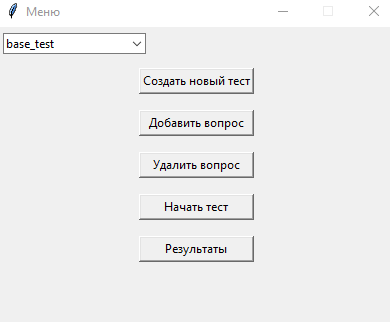
\includegraphics[width=1\linewidth]{menu}
\caption{Композиция шаблона системы}
\label{menu:image}
\end{figure}
%\vspace{-\figureaboveskip} % двойной отступ не нужен (можно использовать, если раздел заканчивается картинкой)

\subsection{Моделирование вариантов использования}

Для разрабатываемой системы тестирования была реализована модель, которая обеспечивает наглядное представление вариантов использования системы.

Она помогает в физической разработке и детальном анализе взаимосвязей объектов.

Диаграмма вариантов описывает функциональное назначение разрабатываемой системы. То есть это то, что система будет непосредственно делать в процессе своего функционирования. Она является исходным концептуальным представлением системы в процессе ее проектирования и разработки. Проектируемая система представляется в виде ряда прецедентов, предоставляемых системой актерам или сущностям, которые взаимодействуют с системой. Актером или действующим лицом является сущность, взаимодействующая с системой извне (например, человек, техническое устройство). Прецедент служит для описания набора действий, которые система предоставляет актеру.

На основании анализа предметной области в программе должны быть реализованы следующие варианты использования:
\begin{enumerate}
\item ВИ "Запустить программу". Данный прецедент позволяет пользователю открыть программу.
\item ВИ "Авторизация". Данный прецедент позволяет пользователю авторизоваться.
\item ВИ "Выбрать желаемый тест". Данный прецедент позволяет пользователю выбрать желаемый тест.
\item ВИ "Пройти выбранный тест". Данный прецедент позволяет пользователю открыть пройти выбранный тест.
\item ВИ "Добавить вопрос". Данный прецедент позволяет пользователю добавить вопрос в выбранном тесте.
\item ВИ "Удалить вопрос". Данный прецедент позволяет пользователю удалить вопрос в выбранном тесте.
\item ВИ "Просмотреть результаты". Данный прецедент позволяет пользователю посмотреть результаты предыдущих тестов.
\item ВИ "Создать новый тест". Данный прецедент позволяет пользователю создать новый тест.
\end{enumerate}

Диаграмма прецедентов представлена на рисунке ~\ref{precedent:image}.

\begin{figure}[ht]
	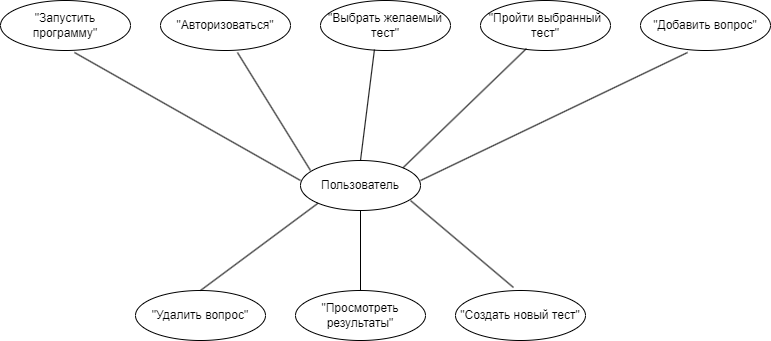
\includegraphics[width=1\linewidth]{precedent}
	\caption{Диаграмма прецедентов}
	\label{precedent:image}
\end{figure}

\subsection{Описание вариантов использования}

Данные варианта использования "Пройти выбранный тест".

Входными данными является выбранный тест, имя пользователя.

Выходными данными прецедента "Пройти выбранный тест" являются вопросы с ответами и результат прохождения теста.

Основной исполнитель: Пользователь.

Заинтересованные лица и их требования: Пользователь хочет пройти тест.

Предусловие: поля для ввода имени, ответа на вопрос должны быть заполнены.

Постусловие: приложение проверит введены ли данные, если нет, сообщит об этом пользователю.

Основной успешный сценарий:
\begin{enumerate}
	\item Пользователь запускает программу.
	\item Пользователь проходит авторизацию, введя своё имя.
	\item Пользователь попадает в меню.
	\item Пользователь выбирает желаемый тест.
	\item Пользователь нажимает кнопку "Пройти тест".
	\item Пользователь попадает в окно теста.
	\item Пользователь выбирает или вводит ответы.
	\item Пользователь по окончании теста видит его результат.
	\item Пользователь закрывает приложение.
\end{enumerate}

Данные варианта использования "Создать новый тест".

Входными данными является имя пользователя.

Выходными данными прецедента "Создать новый тест" являются новый тест с вопросами и ответами.

Основной исполнитель: Пользователь.

Заинтересованные лица и их требования: Пользователь хочет создать тест и добавить в него вопрос

Предусловие: поля для ввода имени, текста вопроса и его ответа должны быть заполнены.

Постусловие: приложение проверит введены ли данные, если нет, сообщит об этом пользователю.

Основной успешный сценарий:
\begin{enumerate}
	\item Пользователь запускает программу.
	\item Пользователь проходит авторизацию, введя своё имя.
	\item Пользователь попадает в меню.
	\item Пользователь выбирает желаемый тест.
	\item Пользователь нажимает кнопку "Создать тест".
	\item Пользователь попадает в окно создания теста".
	\item Пользователь нажимает кнопку "Создать новый тест".
	\item Пользователь нажимает кнопку "Вернуться в меню".
	\item Пользователь попадает в меню.
	\item Пользователь нажимает кнопку "Добавить вопрос".
	\item Пользователь попадает в меню добавления вопроса.
	\item Пользователь нажимает кнопку добавить базовый вопрос.
	\item Пользователь в окне создания базового вопроса вводит текст и ответ вопроса.
	\item Пользователь нажимает кнопку добавить вопрос.
	\item Пользователь закрывает приложение.
\end{enumerate}

\subsection{Требования к оформлению документации}

Разработка программной документации и программного изделия должна производиться согласно ГОСТ 19.102-77 и ГОСТ 34.601-90. Единая система программной документации.
